\section{Identifikácia FIR modelu}
Doteraz sme načrtli situáciu, ako by sme mohli využiť metódu garantovaného odhadu na určenie minimálnej štruktúry modelu a odhad jeho parametrov. Poďme si teraz ukázať ako by sme túto metódu mohli aplikovať na niektorých dátových dynamických modeloch a začneme s FIR modelom.

Najskôr si pripomenieme štruktúru FIR modelu. Ako uvádza rovnica \ref{eq:FIR_m}, FIR model má nasledovný tvar
\begin{equation*}
	\hat{y}(t) = \sum_{i=1}^{n_b} b_{i}u(t-i) = b_{1}u(t-1) + b_{2}u(t-2) + \dots + b_{n_b}u(t-n_b),
\end{equation*}
kde $ n_b $ predstavuje rád modelu, resp. počet parametrov $ b $. 

Aby sme mohli odhadnúť parametre takéhoto modelu, potrebujeme najskôr poznať jeho štruktúru. Na to využijeme metódu odhadu minimálneho rádu modelu, ktorú sme zadefinovali ako \ref{eq:GPE_m_order_est}. V tomto prípade musíme danú formuláciu upraviť do tvaru
\begin{equation}
	\begin{split}
		& \min_{B \in \left[ b_{1}, b_{2}, \dots, b_{n_b} \right]} \quad 0, \\
		& \qquad \quad \text{s.t.} \quad \ubar{e} \leq y - \hat{y} \leq \bar{e}
	\end{split}
	\label{eq:gpe_fir_min_rad}
\end{equation} 
ktorá nám vráti hodnotu minimálneho rádu FIR modelu $ n_b $. V tomto momente už máme k dispozícii informáciu o vyhovujúcej štruktúre modelu, ktorá vyhovuje podmienke GOP. Nasleduje odhad intervalových hodnôt parametrov. Tie získame modifikáciou rovnice \ref{eq:gpe:general_form}
\begin{equation}
	\begin{split}
		\left[ \ubar{b}_i, \bar{b}_i \right] = \min_{B \in \left[ \ubar{b}, \bar{b} \right]} / &\max_{B \in \left[ \ubar{b}, \bar{b} \right]} \quad b_i,\\
		\text{s.t.}& \quad \ubar{e} \leq y - \hat{y} \leq \bar{e}	
	\end{split}
	\label{eq:gpe_fir_param_est}
\end{equation}
pre všetky $ i = 1, 2, \dots, n_b $.  

Týmto sme ukončili identifikáciu FIR modelu minimálneho rádu a v ďalšom postupe by sme sa mali venovať overovaniu správnosti a posudzovaniu kvality daného modelu a modelov vyššieho rádu.

\section{Identifikácia ARX modelu}
ARX model, ako opisuje rovnica \ref{eq:ARX_m}, má štruktúru doplnenú o člen $ A(q) $ oproti FIR modelu a má tvar
\begin{equation*}
	\begin{split}
		\hat{y}(t) &= \frac{\sum_{i=1}^{n_b} b_{i}u(t-i)}{1 + \sum_{i=1}^{n_a} a_{i}q^{-i}} =\\
		&= -a_{1}\hat{y}(t-1) - \dots -a_{n_a}\hat{y}(t-n_a) + b_{1}u(t-1) + \dots + b_{n_b}u(t-n_b).
	\end{split}
\end{equation*}
Výhodou ARX modelu je, že dokáže drasticky znížiť počet parametrov oproti FIR modelu, kvôli príspevku minulých výstupov $ \hat{y}(t-i) $. Avšak, v porovnaní s identifikáciou FIR modelu, je identifikácia ARX modelu omnoho zložitejšia problematika. Práve príspevok minulých výstupov nám transformuje optimalizačnú úlohu z jednoduchej lineárnej (ako to bolo pri identifikácii FIR modelu) na zložitú nelineárnu. V každom prípade postup identifikácie ostáva rovnaký. Najskôr určíme minimálnu štruktúru ARX modelu, ktorá spĺňa podmienky GOP a v ďalšom kroku odhadneme jej parametre resp. intervalové hodnoty parametrov. 

Minimálnu štruktúru ARX modelu, teda rád čitateľa $ n_b $ a rád menovateľa $ n_a $, nájdeme ako riešenie danej optimalizačnej úlohy
\begin{equation}
	\begin{split}
		\min_{a_{1},\dots,a_{n_a},b_{1},\dots,b_{n_b},\hat{y}(t)} & \quad 0.\\
		\text{s.t.} \qquad \quad  & \quad \ubar{e} \leq y - \hat{y} \leq \bar{e} \\
		& \quad \hat{y}(0) = \hat{y}_{0}
	\end{split}
	\label{eq:gpe_arx_min_rad}
\end{equation}
A odhad intervalových hodnôt parametrov určíme ako
\begin{equation}
	\begin{split}
		\left[ \ubar{\theta}_i, \bar{\theta}_i \right] = \min_{\Theta \in \left[ \ubar{\theta}, \bar{\theta} \right]} / \max_{\Theta \in \left[ \ubar{\theta}, \bar{\theta} \right]} & \quad \theta_i,\\
		\text{s.t.} \qquad & \quad \ubar{e} \leq y - \hat{y} \leq \bar{e}\\
		& \quad \hat{y}(0) = \hat{y}_{0}
	\end{split}
	\label{eq:gpe_arx_param_est}
\end{equation}
pre všetky $ i = 1,2, \dots, n_a+n_b $ a $ \Theta $ predstavuje vektor minimálnych a maximálnych hodnôt parametrov $ a, b $
\begin{equation*}
	\Theta = 
	\begin{pmatrix}
		\ubar{a}_{1} & \bar{a}_{1}\\
		\ubar{a}_{2} & \bar{a}_{2}\\
		\vdots & \vdots\\
		\ubar{a}_{n_a} & \bar{a}_{n_a}\\
		\ubar{b}_{1} & \bar{b}_{1}\\
		\ubar{b}_{2} & \bar{b}_{2}\\
		\vdots & \vdots\\
		\ubar{b}_{n_b} & \bar{b}_{n_b}\\	
	\end{pmatrix}.
\end{equation*}
Zložitosť týchto optimalizačných úloh je pravdepodobne očividná, ale pre rozumné rády modelov, táto optimalizácia nemusí byť nutne náročná. Rozdiel v identifikácii ARX modelu spočíva v tom, že musíme v každom nameranom bode odhadovať hodnotu $ \hat{y}(t) $, čo nám pridáva na počte odhadovaných parametrov.

\section{Príklady identifikácie}
V tejto časti si na konkrétnom príklade ukážeme identifikáciu FIR aj ARX modelu. Začnime tým, že si zadefinujeme problematiku. Predstavme si, že sme z neznámeho procesu získali údaje o vstupoch a výstupoch, tak ako je znázornené na Obr. \ref{fig:gpe_tf_ex_data}, ktoré sú v skutočnosti opísané prenosovou funkciou 1. rádu so zosilnením $ K = 8 $ a časovou konštantou $ T = 2 $
\begin{equation*}
	G(s) = \frac{K}{Ts + 1} = \frac{8}{2s + 1}.
\end{equation*}
Tak ako všetky reálne dáta, výstupné údaje sú zaťažené šumom, a presnosť merania senzora je $ e = \pm 0.8 $. 
\begin{figure}
	\centering
	\begin{subfigure}[b]{0.48\textwidth}
		\centering
		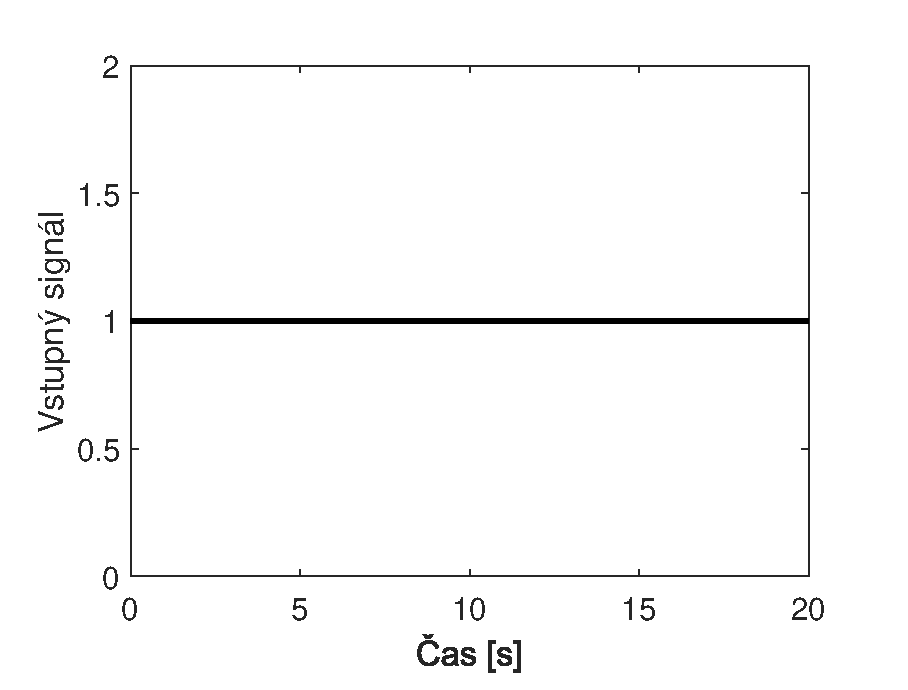
\includegraphics[width=\linewidth]{images/gpe_tf_ex_input}
		\caption{Vstupné údaje}
	\end{subfigure}
	\begin{subfigure}[b]{0.48\textwidth}
		\centering
		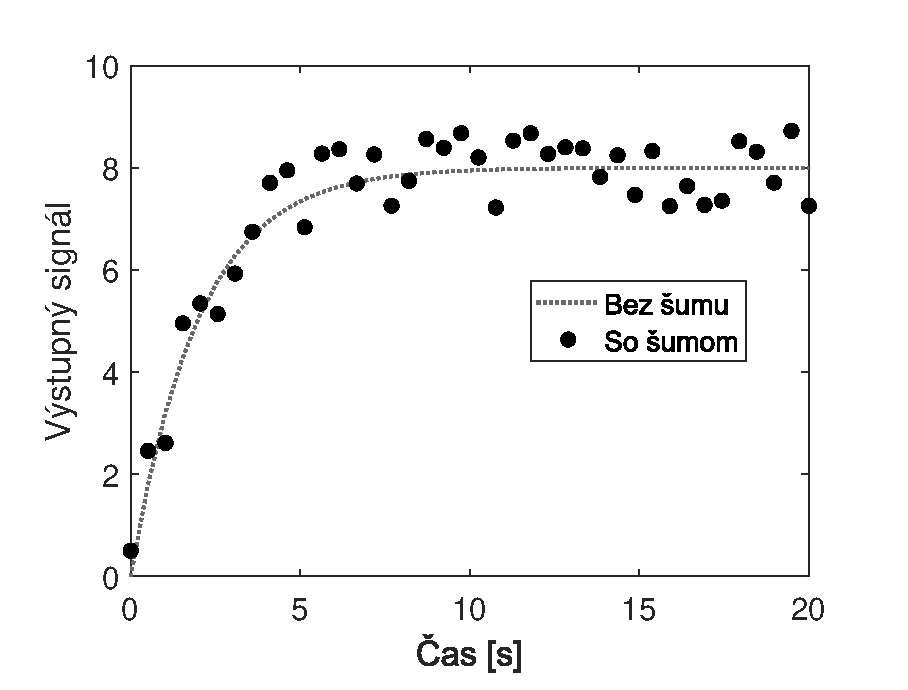
\includegraphics[width=\linewidth]{images/gpe_tf_ex_output}
		\caption{Výstupné údaje}
	\end{subfigure}
	\caption{Namerané dáta z procesu opísaného prenosovou funkciou 1. rádu so zosilnením $ K = 8 $ a časovou konštantou $ T = 2 $.}
	\label{fig:gpe_tf_ex_data}
\end{figure}

Výsledok identifikácie FIR modelu môžeme vidieť na Obr. \ref{fig:gpe_tf_ex_FIRident}. Minimálna veľkosť modelu, ktorá dokázala vhodne opísať dané dáta v stanovej chybe merania, bola $ n_b = 11 $. Ako ukazuje Pareto front na Obr. \ref{fig:gpe_tf_ex_FIRpareto}, tak tento rád modelu je aj najvhodnejším na opis nameraných údajov. V tomto prípade sme dali do pomeru presnosť odhadu a maximálny rozptyl odhadu modelu, pričom hodnoty oboch vlastností sú vztiahnuté na výsledky dosiahnuté modelom 11. rádu.
\begin{figure}
	\centering
	\begin{subfigure}[b]{0.48\textwidth}
		\centering
		\includegraphics[width=\linewidth]{images/gpe_tf_ex_FIRpareto}
		\caption{Pareto front.}
		\label{fig:gpe_tf_ex_FIRpareto}
	\end{subfigure}
	\begin{subfigure}[b]{0.48\textwidth}
		\centering
		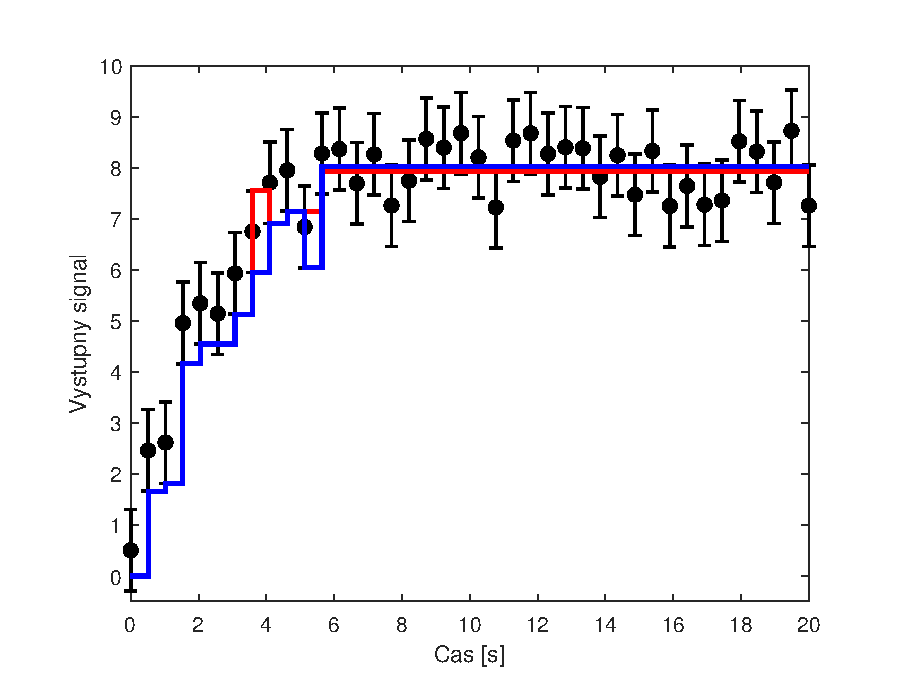
\includegraphics[width=\linewidth]{images/gpe_tf_ex_FIRident}
		\caption{Identifikácia FIR modelu.}
		\label{fig:gpe_tf_ex_FIRident}
	\end{subfigure}
	\caption{Výsledok identifikácie FIR modelu ($ n_b = 11 $) --- minimálna realizácia (červená), maximálna realizácia (modrá), namerané údaje s danou chybou merania (čierna). Čísla pod ukazovateľmi Pareto frontu vyjadrujú rád FIR modelu.}
	\label{fig:gpe_tf_ex_FIR}
\end{figure}

Po intervalovom odhade parametrov sme získali FIR v nasledovnom tvare
\begin{equation*}
	\begin{split}
		\hat{y}(t) \quad = \quad &[1.6587, 3.2587]u(t-1) + [-1.4459, 1.7541]u(t-2) + \\
		 + &[0.7417, 3.9417]u(t-3) + [-1.2112, 1.9888]u(t-4) + \\
		 + &[-1.8069, 1.3931]u(t-5) + [-0.8084, 2.3916]u(t-6) + \\
		 + &[-0.7821, 2.4179]u(t-7) + [-0.6424, 2.5576]u(t-8) + \\
		 + &[-1.3556, 1.8444]u(t-9) + [-2.7116, 0.4884]u(t-10) + \\
		 + &[0.2836, 1.9842]u(t-11).
	\end{split}
\end{equation*}

Výstup identifikácie ARX modelu môžeme vidieť na Obr. \ref{fig:gpe_tf_ex_ARXident}. Minimálna štruktúra bola opísaná diferenčnou rovnicou procesu 1. rádu a podobne ako pri identifikácii FIR modelu, takáto štruktúra ARX modelu je aj najvhodnejšou na opis nameraných dát. To nám potvrdzuje aj Pareto front, ktorý je zobrazený na Obr. \ref{fig:gpe_tf_ex_ARXpareto}. Treba zdôrazniť fakt, že modely vyššieho rádu sú po kvalitatívnej stránke modelu výrazne horšie v porovnaní s ARX modelom 1. rádu.

Po odhade intervalových hodnôt parametrov, sme získali model v tvare
\begin{equation*}
	\hat{y}(t) = [0.7581, 0.7840]\hat{y}(t-1) + [1.7396, 1.9155]u(t-1).
\end{equation*}

\begin{figure}
	\centering
		\centering
	\begin{subfigure}[b]{0.48\textwidth}
		\centering
		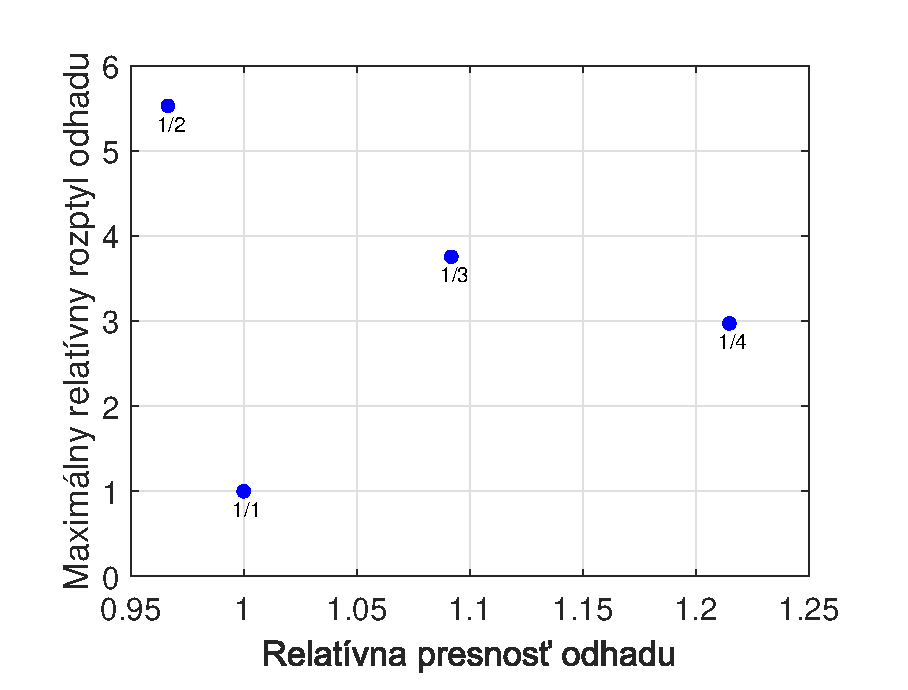
\includegraphics[width=\linewidth]{images/gpe_tf_ex_ARXpareto}
		\caption{Pareto front.}
		\label{fig:gpe_tf_ex_ARXpareto}
	\end{subfigure}
	\begin{subfigure}[b]{0.48\textwidth}
		\centering
		\includegraphics[width=\linewidth]{images/gpe_tf_ex_ARXident}
		\caption{Identifikácia ARX modelu.}
		\label{fig:gpe_tf_ex_ARXident}
	\end{subfigure}
	\caption{Výsledok identifikácie ARX modelu ($ n_b = 1, n_a = 1 $) --- minimálna realizácia (červená), maximálna realizácia (modrá), namerané údaje s danou chybou merania (čierna). Čísla pod ukazovateľmi Pareto frontu vyjadrujú rád ARX modelu v tvare $ \frac{n_b}{n_a} $.}
	\label{fig:gpe_tf_ex_ARX}
\end{figure}

Rozdiel v zložitosti modelov je očividný, avšak v oboch prípadoch sme získali oblasť riešení, ktorá nám garantuje, že skutočné riešenie leží niekde vo vnútri. Táto oblasť je definovaná kombináciou minimálnych resp. maximálnych parametrov, ktoré nám zabezpečia spodné (minimálna realizácia) resp. horné (maximálna realizácia) ohraničenie. Treba taktiež spomenúť, že nie sme odkázaný iba na intervalový odhad. Akonáhle získame informáciu o štruktúre modelu, môžeme využiť napríklad metódu najmenších štvorcov (MNŠ) na identifikáciu neznámych parametrov. 
